\documentclass[aspectratio=169]{beamer}
\hypersetup{pdfpagemode=FullScreen}
\usepackage[utf8]{inputenc}
\usepackage[T1]{fontenc}
\usepackage{lmodern}
\usepackage[english]{babel}
\usepackage{graphicx}
\usepackage{amsmath}
\usepackage{amsfonts}
\usepackage{amssymb}
%\usetheme{CambridgeUS}
%\usetheme{Berlin}
%\usetheme{Montpellier}
\usetheme{Boadilla}
\useinnertheme{circles}
\renewcommand{\footnotesize}{\fontsize{6pt}{10pt}\selectfont}
%\usepackage[nottoc]{tocbibind}
\usepackage{cite}
%\useoutertheme{miniframes} % Alternatively: miniframes, infolines, split
%\useinnertheme{circles}
%\usecolortheme{default}
%\usecolortheme{dolphin}
\usepackage{hyperref}
\usefonttheme[onlymath]{serif}
\setbeamertemplate{caption}[numbered]
\setbeamertemplate{bibliography item}{\insertbiblabel}
%\hypersetup{
%	colorlinks=true,
%	linkcolor=blue,
%	filecolor=magenta,      
%	urlcolor=cyan,
%}
\renewcommand{\figurename}{Fig.}
\setbeamertemplate{section in toc}[sections numbered]
\insertsectionnavigationhorizontal{.5\textwidth}{\hskip0pt plus1filll}{}
%\setbeamertemplate{frametitle}[rounded]
\setbeamertemplate{blocks}[rounded][shadow]



\defbeamertemplate*{footline}{CambridgeUS theme}
{
	\leavevmode%
	\hbox{%
		\begin{beamercolorbox}[wd=.333333\paperwidth,ht=2.25ex,dp=1ex,center]{author in head/foot}%
			\usebeamerfont{author in head/foot}%\insertshortauthor
			~~\insertshortinstitute
		\end{beamercolorbox}%
		\begin{beamercolorbox}[wd=.333333\paperwidth,ht=2.25ex,dp=1ex,center]{title in head/foot}%
			\usebeamerfont{title in head/foot}\insertshorttitle
		\end{beamercolorbox}%
		\begin{beamercolorbox}[wd=.333333\paperwidth,ht=2.25ex,dp=1ex,right]{date in head/foot}%
			\usebeamerfont{date in head/foot}\hspace*{2em}
			Slide: \insertframenumber{} of \inserttotalframenumber\hspace*{2ex}
	\end{beamercolorbox}}%
	\vskip0pt%
}



\defbeamertemplate*{headline}{CambridgeUS theme}
{
	\leavevmode%
	\hbox{%
		\begin{beamercolorbox}[wd=.333333\paperwidth,ht=2.25ex,dp=1ex,center]{author in head/foot}%
			\usebeamerfont{author in head/foot}%\insertshortauthor
			~~%\insertshortinstitute
		\end{beamercolorbox}%
		\begin{beamercolorbox}[wd=.333333\paperwidth,ht=2.25ex,dp=1ex,center]{title in head/foot}%
			\usebeamerfont{title in head/foot}%\insertshorttitle
		\end{beamercolorbox}%
		\begin{beamercolorbox}[wd=.333333\paperwidth,ht=2.25ex,dp=1ex,right]{date in head/foot}%
			\usebeamerfont{date in head/foot}\insertshortdate{}\hspace*{2em}
			\textsl{\emph{{{{\tiny {\tiny }}}}}}%\insertframenumber{} of \inserttotalframenumber\hspace*{2ex}
	\end{beamercolorbox}}%
	\vskip0pt%
}

  
  
  \definecolor{UniBlue}{RGB}{83,121,170}
  
  \setbeamercolor{title}{fg=white, bg=UniBlue}
  %\setbeamercolor{title in head/foot}{fg=black,bg=lightgray}
  %\setbeamercolor{author in head/foot}{fg=white,bg=black}
 %\setbeamercolor{frametitle}{fg=white,bg=black}
  %\setbeamercolor{block title}{fg=white,bg=black}
  %\setbeamercolor{block body}{bg=lightgray, fg=black}
  %\setbeamercolor{date in head/foot}{fg=white, bg=black}
  %\setbeamercolor{item}{fg=gray}
  




  
\begin{document}
	%\author{}
	\title{Power Distribution System for a CubeSat}
	
	\subtitle{}
	%\logo{}

	
     \author{Presented by :\\Ansaf Niyaz | TRV19EE016  \and Govind Murali | TRV19EE025  \and \\Jijesh J. Kumar | TRV19EE029  \and Naveen A.B. | TRV19EE038}

	\institute{GEC Barton Hill,Thiruvananthapuram}
	\date{\today}
	
	
	\setbeamercovered{transparent}
\setbeamertemplate{navigation symbols}
{%
	\hbox{%
		\hbox{\insertslidenavigationsymbol}
		\hbox{\insertframenavigationsymbol}
		\hbox{\insertsubsectionnavigationsymbol}
		\hbox{\insertsectionnavigationsymbol}
		\hbox{\insertdocnavigationsymbol}
		\hbox{\insertbackfindforwardnavigationsymbol}}%
}
	\begin{frame}[plain]
	\maketitle
	\center{Guided by: Prof. Dinesh Gopinath}
%	\center{{SEMINAR PRESENTATION}}
\end{frame}


\begin{frame}
\frametitle{Contents}




\tableofcontents
\end{frame}



\section{Objectives}
\begin{frame}
	
\frametitle{Objective}
 To design and implement a fully autonomous power generation, storage and distribution system for a CubeSat 
 
 

\end{frame}




\section{Project Outline}

\begin{frame}
	\frametitle{Project Outline	}

	\begin{minipage}{0.5\textwidth}
	CubeSat(1U):
\begin{itemize}
	
	\item Dimensions-10x10x10 cm 
	\item Weight-2 kg.
\end{itemize}
\end{minipage}
\begin{minipage}{0.3\textwidth}
		\begin{figure}
	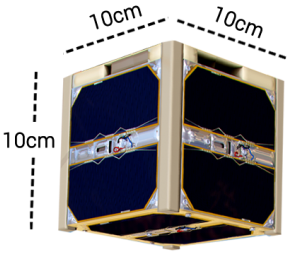
\includegraphics[width=5.1cm]{cubes1.png}
	\begin{center}
		\caption{CubeSat 1U (Source: GIS Geography )}
	\end{center}
	\label{fig:trac2}
	
\end{figure}
	
\end{minipage}

	 \end{frame}


\begin{frame}
	\frametitle{Project Outline (Contd.)}
 	Electrical Power System (EPS):
 	\begin{itemize}
 		
 		\item Harvests energy from the solar panels
 		\item Manages power storage and distribution
 		\item Protects circuits from damage
 		\item Redundant architecture
 	\end{itemize}
\end{frame}


\section{System Architecture}
\begin{frame}{System Architecture}
	
	

	
\end{frame}

\section{Methodology}

	
	
	
	

\begin{frame}{Methodology}
		\begin{itemize}
			
			\item Identifying the power requirements
			\item Literature Review
			\item Forming Specifications
			\item Architecture design and topology selection
			\item Design and simulation
			\item Procurement of components
			\item Fabrication and testing
		
		\end{itemize} 
	
\end{frame}


\section{Requirements}
\begin{frame}{Requirements}
	\begin{minipage}{0.5\textwidth}
		Equipments Requirements:
		\begin{itemize}
			
			\item SMD Soldering Station
			\item Oscilloscope
			\item Power Supply
			\item Function Generator
		\end{itemize} 
	\end{minipage}
	\begin{minipage}{0.3\textwidth}
		Software Requirements:
		\begin{itemize}
			
			\item MATLAB/Spice
			\item KiCad
			\item STM32 CubeIDE
			
		\end{itemize} 
		
	\end{minipage}
\end{frame}



\section{Budget Estimate: Component cost}
\begin{frame}{Budget Estimate: Component cost}

\begin{table}[]
	\begin{tabular}{|l|l|l|l}
		\cline{1-3}
		\textbf{Sl. No.} & \textbf{Item}                       & \textbf{Amount (Rs.)} &  \\ \cline{1-3}
		1                & STM32 NUCLEO Development Board      & 3000                  &  \\ \cline{1-3}
		2                & SMD soldering station               & 9000                  &  \\ \cline{1-3}
		3                & Li - ion Cell (x2)                  & 1000                  &  \\ \cline{1-3}
		4                & Regulated Multi-Output Power Supply & 5000                  &  \\ \cline{1-3}
		5                & Solar Cell                          & 10000                    &  \\ \cline{1-3}
		6                & Components                          & 5000+shipping         &  \\ \cline{1-3}
	\end{tabular}
\end{table}

		

\end{frame}

\section{Budget Estimate: Fabrication cost}
\begin{frame}{Budget Estimate: Fabrication cost}
\begin{table}[]
	\begin{tabular}{|l|l|l|l}
		\cline{1-3}
		\textbf{Sl. No.} & \textbf{Item}        & \textbf{Amount (Rs.)} &  \\ \cline{1-3}
		1                & PCB Printing         & ??                    &  \\ \cline{1-3}
		2                & SMD soldering        & ?                     &  \\ \cline{1-3}
		3                & Inductor Fabrication & 1000                  &  \\ \cline{1-3}
	\end{tabular}
\end{table}
\end{frame}


\begin{frame}[allowframebreaks]{References}

\begin{thebibliography}{9}
	
		\bibitem[1]{p1}
Moraes, Caio Guilherme da Silva and Brockveld, Sergio Luis and Heldwein, Marcelo Lobo and Franca, André Stanzani and Vaccari, Anderson Silva and Waltrich, Gierri (2021)
\newblock Power Conversion Technologies for a Hybrid Energy Storage System in Diesel-Electric Locomotives
\newblock \emph{IEEE Transactions on Industrial Electronics}  vol. 68, no. 10, pp. 9081-9091.

	 % Reduce the font size in the bibliography

\end{thebibliography}
\end{frame}

\begin{frame}
	\begin{columns}
		\column{2.5cm}
		\column{5cm}
		\Huge{~}
		\column{2.5cm}
	\end{columns}
\end{frame}
%\end{frame}
\end{document}